\documentclass[a4paper,11pt]{article}
\usepackage{graphicx}
\usepackage{enumerate}

\begin{document}

\begin{flushright}

\vspace{1.1cm}

{\bf\Huge Problem Set 3}

\rule{0.25\linewidth}{0.5pt}

\vspace{0.5cm}
%Put Authors
Justin Ely
\linebreak
\newline
%Put Author's affiliations
\footnotesize{605.411 Foundations of Computer Architecture \\}
\vspace{0.5cm}
% Date here below
20 September, 2016
\end{flushright}

\noindent\rule{\linewidth}{1.0pt}

%%%%%%%%%%%%%%%%%%%%%%%%%%%%%%%%%%%%%%%%%%%%%%%%%%%%%%%%%%

\section*{1)}
For this, and following solutions, (n) represents column n in the table.  This is used to reduce errors in typing when doing
arithmetic with derived columns. \\

\begin{tabular}{| l | c | c | c | c | c | c | c | c |}
  \hline	
    1 & 2 & 3 & 4 & 5 & 6 & 7  \\  \hline \hline
    a & b & (ab)' & A'(3) & B'(3) & ((4)(5))' & ((6)(6))'  \\  \hline \hline
    0 & 0 & 1 & 1 & 1 & 0 & 1  \\  \hline 
    1 & 0 & 1 & 0 & 1 & 1 & 0  \\  \hline 
    0 & 1 & 1 & 1 & 0 & 1 & 0  \\  \hline 
    1 & 1 & 0 & 1 & 1 & 0 & 1  \\  \hline 
\end{tabular} \\

\noindent  The result (column 7) has the same truth table as a XNOR gate.

%%%%%%%%%%%%%%%%%%%%%%%%%%%%%%%%%%%%%%%%%%%%%%%%%%%%%%%%%%

\section*{2)} 
\begin{tabular}{| l | c | c | c | c | c | c | c | c |}
  \hline	
    ROW & A & B & C & Y & Maxterm & Minterm  \\  \hline \hline
    0 & 0 & 0 & 0 & 1 &  &   A'B'C' \\  \hline 
    1 & 0 & 0 & 1 & 0 & A + B + C' &   \\  \hline 
    2 & 0 & 1 & 0 & 1 &  & A'BC'  \\  \hline 
    3 & 0 & 1 & 1 & 1 &  &  A'BC \\  \hline 
    4 & 1 & 0 & 0 & 0 & A' + B + C &   \\  \hline 
    5 & 1 & 0 & 1 & 0 & A' + B + C' &   \\  \hline 
    6 & 1 & 1 & 0 & 1 &  &  ABC' \\  \hline 
    7 & 1 & 1 & 1 & 0 & A' + B' + C' &   \\  \hline 
\end{tabular} \\

%%%%%%%%%%%%%%%%%%%%%%%%%%%%%%%%%%%%%%%%%%%%%%%%%%%%%%%%%%

\section*{3a)}
\begin{tabular}{| l | c | c | c | c | c | c | c | c |}
  \hline	
    1 & 2 & 3 & 4 & 5 & 6 & 7  \\  \hline \hline
    a & b & c & ab & bc & ac & (4) + (5) + (6)  \\  \hline \hline
    0 & 0 & 0 & 0 & 0 & 0 & 0  \\  \hline 
    0 & 0 & 1 & 0 & 0 & 0 & 0  \\  \hline 
    0 & 1 & 0 & 0 & 0 & 0 & 0  \\  \hline 
    0 & 1 & 1 & 0 & 1 & 0 & 1  \\  \hline 
    1 & 0 & 0 & 0 & 0 & 0 & 0  \\  \hline 
    1 & 0 & 1 & 0 & 0 & 1 & 1  \\  \hline 
    1 & 1 & 0 & 1 & 0 & 0 & 1  \\  \hline 
    1 & 1 & 1 & 1 & 1 & 1 & 1  \\  \hline 
\end{tabular} \\

\section*{3b)}
AB + BC + AC

%%%%%%%%%%%%%%%%%%%%%%%%%%%%%%%%%%%%%%%%%%%%%%%%%%%%%%%%%%

\section*{4)}
\begin{tabular}{| l | c | c | c | c | c | c | c | c |}
  \hline	
    1 & 2 & 3 & 4 & 5 & 6  \\  \hline \hline
    a & b & ab & a'b'& (3) + (4) & (5)'  \\  \hline \hline
    0 & 0 & 0 & 1 & 1 & 0   \\  \hline 
    1 & 0 & 0 & 0 & 0 & 1   \\  \hline 
    0 & 1 & 0 & 0 & 0 & 1   \\  \hline 
    1 & 1 & 1 & 0 & 1 & 0   \\  \hline 
\end{tabular} \\

\noindent This logic circuit can be replaced with a single XOR gate.

%%%%%%%%%%%%%%%%%%%%%%%%%%%%%%%%%%%%%%%%%%%%%%%%%%%%%%%%%%

\section*{5)}
From the circuit diagram shown:

\begin{enumerate}
  \item $o_3 = S`I_2$
  \item $o_2 = SI_3 + S`I_1$
  \item $o_1 = I_2S + S`I_0$
  \item $o_0 = I_1S$
\end{enumerate}

\noindent Thus, by setting $S=1$, and $I_3, I_2 , I_1, I_0 = 1011$, the circuit comes out as: $o_3, o_2, o_1, o_0 = 0101$.

%%%%%%%%%%%%%%%%%%%%%%%%%%%%%%%%%%%%%%%%%%%%%%%%%%%%%%%%%%

\section*{6)}

From problem 1, column 6 is the same output as an XOR gate, and has been constructed with only NAND gates.  Thus, the circuit
would look like that shown in the figure below.

\begin{figure}[h]
\caption{Circuit diagram for an XOR gate using only NAND gates.}
\centering
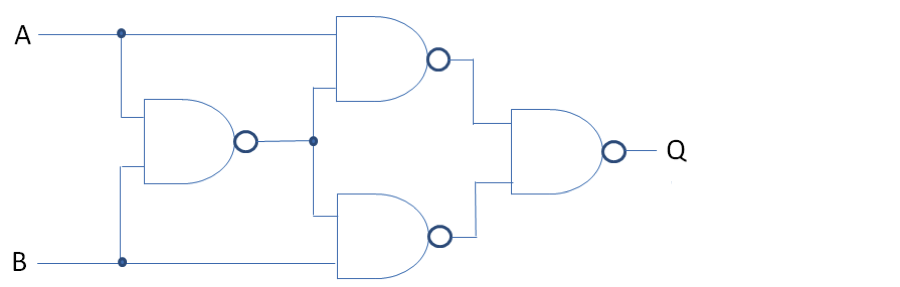
\includegraphics[width=1\textwidth]{p6_circuit.png}
\end{figure}

%%%%%%%%%%%%%%%%%%%%%%%%%%%%%%%%%%%%%%%%%%%%%%%%%%%%%%%%%%

\section*{7)}
\begin{tabular}{| l | c | c | c | c | c | c | c | c |}
  \hline	
    1 & 2 & 3 & 4 & 5 & 6 & 7 & 8 & 9  \\  \hline \hline
    A & B & A`B & AB` & A`B + AB' & C & (5)`C & C'(5) & R  \\  \hline \hline
    0 & 0 & 0 & 0 & 0 & 0 & 0 & 0 & 0  \\  \hline 
    0 & 0 & 0 & 0 & 0 & 1 & 1 & 0 & 1  \\  \hline 
    0 & 1 & 1 & 0 & 1 & 0 & 0 & 1 & 1  \\  \hline 
    0 & 1 & 1 & 0 & 1 & 1 & 0 & 0 & 0  \\  \hline 
    1 & 0 & 0 & 1 & 1 & 0 & 0 & 1 & 1  \\  \hline 
    1 & 0 & 0 & 1 & 1 & 1 & 0 & 0 & 0  \\  \hline 
    1 & 1 & 0 & 0 & 0 & 0 & 0 & 0 & 0  \\  \hline 
    1 & 1 & 0 & 0 & 0 & 1 & 1 & 0 & 1  \\  \hline 

\end{tabular} \\

%%%%%%%%%%%%%%%%%%%%%%%%%%%%%%%%%%%%%%%%%%%%%%%%%%%%%%%%%%

\section*{8a)}
\begin{tabular}{| l | c | c | c | c | c | c | c | c |}
  \hline	
    A & B & C & Z & Minterm \\  \hline \hline
    0 & 0 & 0 & 1 & A'B'C'  \\  \hline
    0 & 0 & 1 & 0 & A'B'C  \\  \hline
    0 & 1 & 0 & 0 & A'BC'  \\  \hline
    0 & 1 & 1 & 1 & A'BC  \\  \hline
    1 & 0 & 0 & 1 & AB'C'  \\  \hline
    1 & 0 & 1 & 0 & AB'C  \\  \hline
    1 & 1 & 0 & 0 & ABC'  \\  \hline
    1 & 1 & 1 & 1 & ABC  \\  \hline
\end{tabular} \\

The function Z is then built of the minterms on rows where Z=1:  $Z = A'B'C' + A'BC + AB'C' + ABC$.

\section*{8b)}
\begin{eqnarray}
Z &=& A'B'C' + A'BC + AB'C' + ABC \\
Z &=& B'C'(A' + A) + BC(A' + A) \\
Z &=& B'C' + BC 
\end{eqnarray}


%%%%%%%%%%%%%%%%%%%%%%%%%%%%%%%%%%%%%%%%%%%%%%%%%%%%%%%%%%

\section*{Appendix}
Jupyter notebook with python code showing verification of problems is attached:

\end{document}
